\documentclass[a4paper,article,11pt,oneside]{article}
\usepackage{graphicx}
\usepackage{url}

\begin{document}
\title{Report for OS Project \#0 (2011 Fall)\\Team 071}
\author{Jeehoon Kang\\\texttt{jhkang@ropas.snu.ac.kr}\and Jonghyuk Lee\\\texttt{jonghyuk0605@gmail.com} \and Taekwon Lee\\\texttt{tkwonlee@hotmail.com} }
\maketitle

This article is structured as follows. Section~\ref{secbochs} briefly
introduces Bochs IA-32 emulator\cite{bochs}; Section~\ref{secpintos},
Pintos operating system framework for
80x86\cite{pintos}. Section~\ref{secinstall} shows the installation
procedure and section~\ref{secexample} presents some running
instances.

\section{Bochs}\label{secbochs}
There are several types of virtualization such as full
virtualization, paravirtualization, and OS-level virtualization. Full
virtualization emulates hardwares so that OS can be installed without
modification. Paravirtualization needs OS to be modofied, but it
presents generally better performance. In OS-level virtualization
model, only one OS kernel is used, but several environments are
provided.

Three types of virtualization are three answers to the trade-off
between generality and performance, full virtualization being the most
general solution and OS-level virtualization being the most performant
solution.

Bochs\cite{bochs}, an IA-32 emulator which supports ``Intel x86 CPU,
common I/O devices, and a custom BIOS,'' is an instance of full
virtualization.\cite{bochs} So it can run major x86 operating systems
including Linux and Windows without modification.

Out of competitors in full virtualization including VMware,
VirtualBox, QEMU, and Parallels, we picked Bochs because it is the most
basic solution and suitable for testing or course projects.

Note that operating systems should behave as emulator-independent; So
hereafter, we focus on OS itself and not on Bochs or other
emulators. Originally this is the reason we picked a full virtual
machine at first.

\section{Pintos}\label{secpintos}
Pintos is an ``operating system framework for 80x86'' from Stanford
University \cite{pintos}. Pintos targets on educations so that it is
highly modular, missing important features to be implemented,
commented for beginners, and well-written. We expect to implement
scheduler, loader, virtual memory, and file systems.

Pintos originated from Nachos an ``instructional software for teaching
undergraduate, and potentially graduate, level operating systems
courses'' from UC Berkeley \cite{nachos}. Their purposes are generally
the same, but Nachos is written in C++ while Pintos is written in C.

Pintos is more suitable for OS course. The reasons are threefold:
first, Pintos it uses the C programming language, more preferable to
C++ in the field of low-level architecture. Second, Nachos targets on
MIPS. Last, Nachos is run as a user process while Pintos is run on top
of an x86 (virtual) machine so Pintos better reflects modern OS
concepts.

Let's see about basic structure and booting process of Pintos.

\subsection{Structure of Pintos}\label{subsecstruc}
The official reference guide in Pintos document explains the structure
of Pintos in detail. In this subsection, we follow the document to
understand structure of Pintos briefly.
\begin{enumerate}
\item Loading\\
\texttt{loader.S} and \texttt{kernel.lds.S} load Pintos and
intialization process to initialize kernel. Detail process will be
described in next subsection.
\item Threads\\
This part supports data structure for threads and utility function for
thread support. Also this part deals with context switching and scheduling.
\item Synchronization\\
Shared resources becomes a problem If multiple threads are
running. Syncronization part resolve that problem. For example, while
a process is running, we might lock I/O of other processes to prevent
undesired behavior.
\item Interrupt Handling\\
An interrupt notifies  CPUs of predefined events such as keyboard
input. Many OS features depend on interrupts so that inturrupt
handling should be an important feature.
\item Memory Allocation\\
Allocating memory is one of important jobs for operating
system. Pintos contains two memory allocators. These are one that
allocates memory in units of a page and one that can allocate blocks
of any size which depends on the allocator on pages.
\item Virtual Adresses\\
Pintos can manage virtual addresses. 32-bit virtual address of Pintos
can be divided into a 20-bit page number and a 12-bit page offset.
\item Page Table\\
This part handles page table. We can create, destruct, and activate
page tables. We also can update and examine page mapping.
\item Hash Table\\
Pintos provides hash table to be used as data structure. For instance, in virtual memory part we can use hash table to translate pages to frames.
\end{enumerate}

\subsection{Booting Process}\label{subsecbooting}
\begin{enumerate}
\item At first, Loader is executed.
\begin{enumerate}
\item PC BIOS loads loader to memory.
\item loader works.
\begin{enumerate}
\item CPUs are initialized (enable A2O line)
\item Asks memory size of PC to BIOS.
\item Make page table. This table maps 64MB in virtual memory.
\item After page table is initialized, loader loads control register
  of CPU and pages in protected mode. It also initializes segment
  register. It can't handle interrupt yet, so it disable interrupt.
\item Finally, loader loads the kernel from disk.
\end{enumerate}
\end{enumerate}
\item Kernel Initialization
\begin{enumerate}
\item \texttt{ram\_init()} initializes kernel RAM. it
\begin{enumerate}
\item clear bss segment, and
\item read size of memory of which has loader.
\end{enumerate}
\item \texttt{main()} reads kernel cmd line and calls \texttt{read\_command\_line()} to parse it. Gets option from \texttt{parse\_option()}.
\item \texttt{thread\_init()} initializes thread system
\item Initializes memory system of kernel. \texttt{palloc\_int()} sets up page allocator. \texttt{malloc\_init()} and \texttt{paging\_init()} is called in order.
\end{enumerate}
\end{enumerate}

\section{Installation}\label{secinstall}
In this section, we presents how we installed Bochs 2.4.6 and
Pintos\footnote{The version is unknown; the TA just gave it to us.} in
Ubuntu 11.04 Desktop edition. We maintain a repository for this and
further projects.\footnote{see
  \texttt{https://ta:ta@147.46.242.9:4431/hg/os}. Unfortunately the
  link is very unreliable.}

We installed both from the source code. Figure~\ref{figinstall}
describes the installation procedure.
\begin{figure}
\begin{verbatim}
cd bochs-2.4.6
./configure --enable-gdb-stub --with-term --with-nogui
make
sudo make install
cd ..

cd pintos/src/threads
make
cd ../../..
\end{verbatim}
\caption{Installation procedure for Bochs and Pintos}\label{figinstall}
\end{figure}

Figure~\ref{figscreenshot} presents the screenshots for the
installation.
\begin{figure}
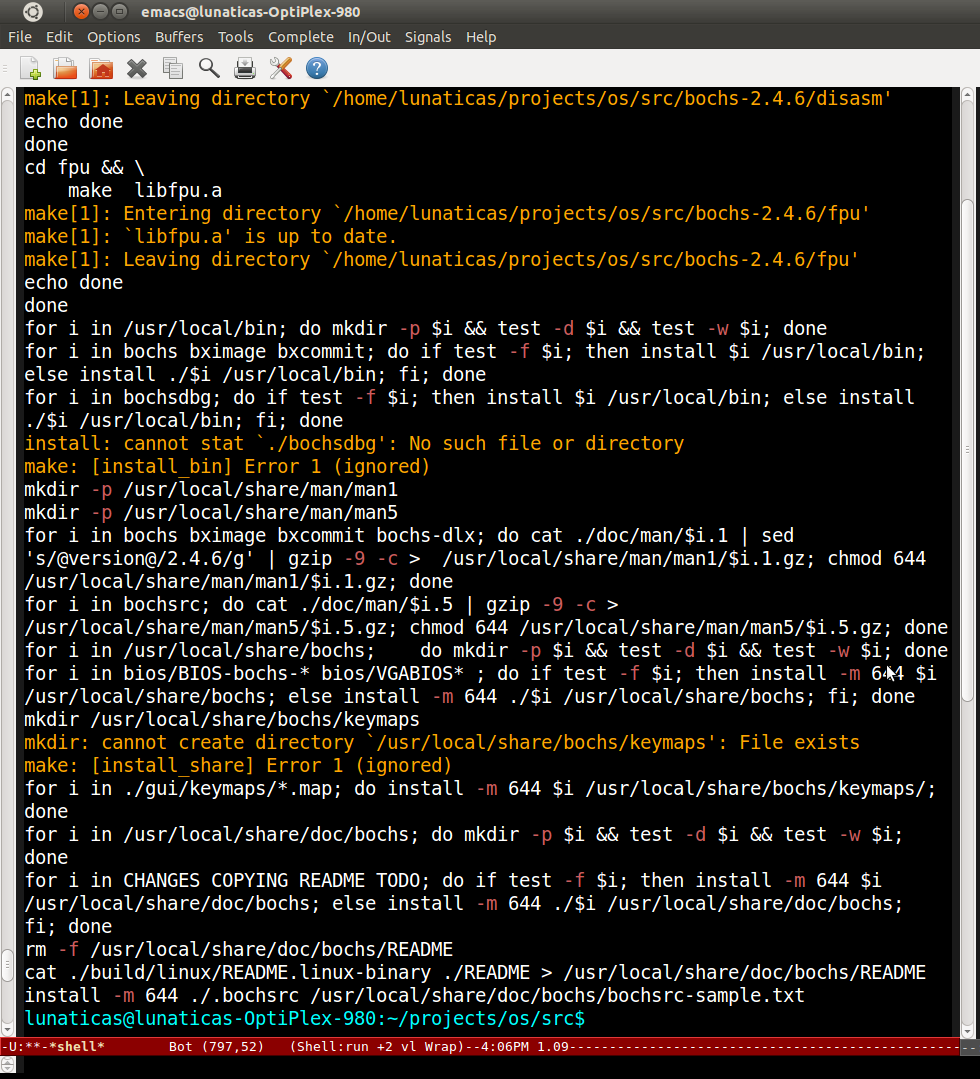
\includegraphics[width=200pt]{bochs.png}
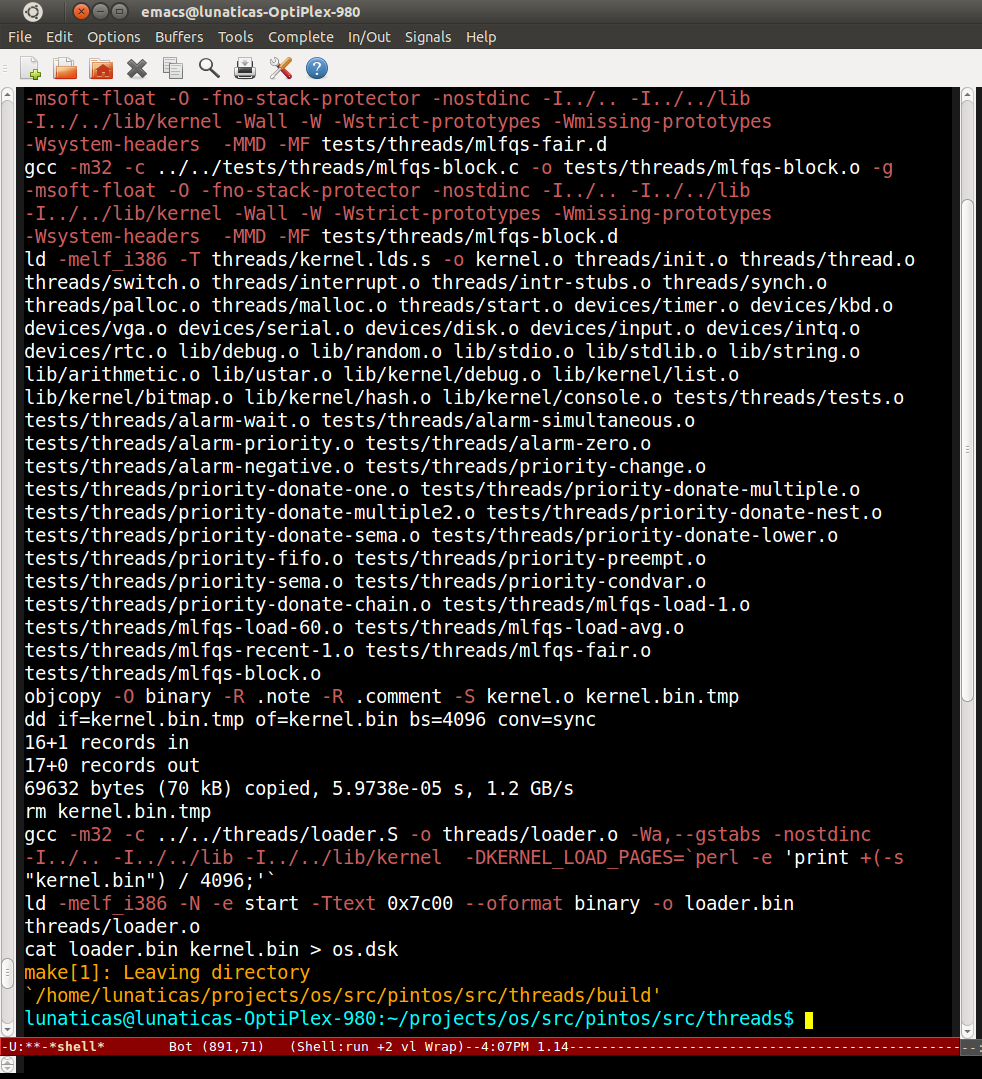
\includegraphics[width=200pt]{pintos.png}
\caption{Screenshots for Bochs and Pintos installation}\label{figscreenshot}
\end{figure}

\section{GDB}\label{secgdb}
Before we start to test pintos with gdb, let's see some common features of gdb.
\begin{enumerate}
\item GDB Command p.
It continues execution until Ctrl+C or the next breakpoint.
\item GDB Command p \textit{expression}.
It evaluates the given expression and prints its value. If the expression contains a function call, that function will actually be executed.
\item GDB Command r.
It runs debugged program. It will be also stopped by signal or break point.(run)
\item GDB Command break \textit{*address}.
Sets a breakpoint at function, at line within file, or address. (Use a “0x” prefix to specify an address in hex.)
Use break main to make GDB stop when Pintos starts running.
\item GDB Command n, s.
n is contraction of "next", Only cursor will point next line(Step Over). s is contraction of "step", it is simillar with n, but it will INTO function if its line contain function.(Step Into)
\item GDB Command l \textit{*address}.
Lists a few lines of code around address. (Use a “0x” prefix to specify an address in hex.)
\item GDB Command b.
Set up a breakpoint.
\item GDB Command bt.
Prints a stack backtrace similar to that output by the backtrace program described above.
\item GDB Command p/a \textit{address}.
Prints the name of the function or variable that occupies address. (Use a “0x” prefix to specify an address in hex.)
\item GDB Command watch \textit{EXP}.
If change of EXP occurs, OLD value and NEW value will be showed.
\item GDB Command disassemble \textit{function}.
Disassembles function. 
\end{enumerate}

In this project, we debug pintos through gdb debugger. At first, we run pintos with \texttt{--gdb} option. Then bochs stops and waits for gdb. Second, open new terminal and run \texttt{gdb kernel.o}.  Finally, command \texttt{target remote localhost:1234} to gdb. Then gdb is connected to pintos through local network connection. After this process, we can use normal gdb commands through it.

\section{Examples}\label{secexample}
In this section, we present two running tests. The second example uses
the GDB debugger.
\begin{itemize}
\item
\begin{verbatim}
cd src/pintos/src/threads/build
../../utils/pintos -- run alarm-multiple
\end{verbatim}
The seperator \texttt{--} separates options and arguments. \texttt{run
  alarm-multiple} instructs to conduct the predefined test.

\item
\begin{verbatim}
cd src/pintos/src/threads/build
../../utils/pintos -t --gdb -s -- run alarm-multiple
\end{verbatim}
\texttt{-t} means terminal; \texttt{--gdb}, gdb debugger; \texttt{-s},
suppressing serial input from stdin and stdout. This is equipped with
debugging funtionalities so that we can debug the program with remote
gdb process.

\end{itemize}

\section{Conclusion}
We made an environment for an OS course. The environment includes
Bochs, Pintos with testing and debugging functionalities, and the
repository for conducting the projects.

\bibliographystyle{plain}
\bibliography{references}
\end{document}
